\section{Introduction}
Thus far, the dissertation has explored perceptual and decisional processes in both perceptual and preferential choice. Experiment 2 showed that stimuli which are more similar to one another, and are thus more easily comparable, generate valuations with stronger correlations. This result holds across both perceptual choice (Chapter 2) and preferential choice (Chapter 4). The comparison process is defined as a cognitive operation where a participant attends to the relative difference between two options on a choice set, typically (though not necessarily) on a single dimension. 

A Thurstonian choice model, conditional on parameters estimated from actual data, can produce the repulsion effect \parencite{spektorWhenGoodLooks2018b,simonson2014vices} because the decoy option, whose value is tightly correlated with the target, occasionally exceeds the target in perceived value and thus takes choice shares away from the target. The model can also predict the attraction effect, but the model with parameters which were estimated from actual empirical data do not predict the attraction effect.

In this chapter, inter-stimulus comparability is manipulated directly in a perceptual choice task. The goal of this manipulation was to empirically test the relationship between comparability and choice. First, the previous literature on comparability is reviewed, and then the results of a perceptual choice experiment are presented.

\subsection{Previous Literature on Comparability}

Other researchers have studied the comparison process in decision-making, particularly in high-level (e.g., preferential) choice. Below, relevant preferential choice research is introduced before transitioning to relevant research on perceptual choice. 

\textcite{changWhichCompromiseOption2008} tested the compromise effect by varying the presentation of options. In the compromise effect, a middle-ground option decreases the choice share of two dissimilar, extreme options. \textcite{changWhichCompromiseOption2008} displayed consumers options in either a by-alternative format, where option names are listed as columns while attribute values are listed as rows, or a by-attribute format, where option attributes are columns while option names are rows. The former display makes it more difficult to compare options on a single attribute, while the latter makes it easier. \textcite{changWhichCompromiseOption2008} found that listing options by-attribute increased the choice share of the compromise option, relative to a by-alternative display. 

\textcite{cataldoComparisonProcessAccount2019b} replicated this result, also finding that a by-alternative format nullified the attraction effect while a by-attribute format strengthens the attraction effect. \textcite{cataldoComparisonProcessAccount2019b} attributed these results to a flexible comparison process, where the comparison strategy is influenced by display format. According to this account, the by-attribute format increases the ease of target-decoy comparisons relative to the by-alternative format. 

\textcite{noguchi2014attraction} studied context effects using eye-tracking, showing that people tend to compare pairs of options on a single attribute, and that these comparisons appear to drive the attraction, similarity, and compromise effect. In \textcite{noguchi2014attraction}'s study, participants' eye movements were more likely to transition between options on a single dimension than they were to transition between dimensions within a single option. Transitions between two options were also negatively related to the choice share of a third option.

\textcite{hayes2024attribute} manipulated attribute comparability, such that the dimensions of each option were either represented in a common unit (high comparability, e.g., 0-10 ratings on all attributes) or in different units (low comparability, e.g., CPU speed vs. RAM for laptops). The attraction effect only occurred in the low comparability condition, with the high comparability condition creating a null effect. The rationale behind this result is that by reducing across-attribute comparability, the researchers are encouraging \textit{within-attribute} comparability, generating the attraction effect in a form similar to \textcite{cataldoComparisonProcessAccount2019b}. 

\textcite{hasan2025registered} conducted a large scale replication study on factors that impact the attraction effect, systematically varying option order, presentation mode (numerical or graphical), and presentation format (by-attribute or by-alternative). \textcite{hasan2025registered} found that the attraction effect was stronger when the target and decoy options were adjacent to one another, presumably because this allows for easier target-decoy comparison. The attraction effect was stronger when attributes were presented numerically compared to graphically, a result found by other researchers \parencite{frederickLimitsAttraction2014b,yangMoreEvidenceChallenging2014}. They did, however, fail to replicate \textcite{cataldoComparisonProcessAccount2019b}'s finding that the attraction effect varies with by-alternative vs. by-attribute format. One possible explanation for this failure to replicate is that \textcite{cataldoFramingContextEffects2020} held absolute TDD constant, while \textcite{hasan2025registered} allowed it to vary with product category. Given that TDD can be a crucial and factor in generating the repulsion effect \textcite{spektorWhenGoodLooks2018b,liaoInfluenceDistanceDecoy2021}, the varied TDDs (and perhaps, limited target-decoy comparability) may have nullified the by-attribute vs. by-alternative difference demonstrated by \textcite{cataldoComparisonProcessAccount2019b}.
% , albeit with different decoy types. In \textcite{cataldoComparisonProcessAccount2019b}'s original study, the decoy was wors

Hsee and colleagues \parencite{hseeEvaluabilityHypothesisExplanation1996,hseeLessBetterWhen1998,hseeWillProductsLook1998,hsee1999preference} have also shown that the comparison of options affects consumer behavior. For example, they repeatedly showed that participants’ evaluation of a given option can change with the addition of a reference point. For example, lower valued options improve with a high reference point and vice versa. Participants’ judgments can reverse when options are evaluated jointly, compared to separately \parencite{hsee1999preference}. 

Several computational models of decision-making also rely on the comparison process.  \textcite{roeMultialternativeDecisionField2001a}'s Multialternative Decision Field Theory (MDFT) model assumes that options accumulate evidence through comparisons on individual attributes, nearby options exhibit greater influence on a given option's preference state than do farther options. According to \textcite{trueblood2014multiattribute}'s Multiattribute Linear Ballistic Accumulator Model (MLBA), each option accumulates evidence through pairwise comparisons to all other available options. These comparisons are modulated by several processes, such as distance in attribute space and extremeness aversion. Other decision models incorporate similar mechanisms \parencite{usherLossAversionInhibition2004a,noguchiMultialternativeDecisionSampling2018a,spektor2019similarity,wollschlager2NaryChoiceTree2012a,landry2021pairwise} (c.f. \textcite{bhatiaAssociationsAccumulationPreference2013b,bergnerVAMPVotingAgent2019b}). 

\textcite{trueblood2022attentional} argued that pairs of similar options garner more attention in the comparison process. They presented a simple Markov model where pairwise comparisons on a single attribute determine the accumulation of preference, and the time spent on a comparison is an increasing function of the similarity of options on the attribute. Their model can successfully, and parsimoniously, account for the attraction, compromise, and similarity effects.

\subsection{Comparability Effects in Perceptual Choice}
There has been other research, albeit relatively limited, studying the comparison process in perceptual choice. Much of this work has focused on the spatial layout of the options and its effect on perceptual context effects.

\textcite{trueblood2022attentional} re-analyzed previous perceptual choice context effect data \parencite{trueblood2015fragile} by examining the order of the options presented to participants. They found that the attraction effect was strongest when the target and decoy were next to each other, while the effect was weak (or even absent) when the options were separated spatially. Their conclusion, supported by a modeling analysis, was that people tend to compare pairs of options which are spatially closer to one another more often than pairs further away from one another. 

\textcite{evansImpactPresentationOrder2021} found a similar result in perceptual choice, though in their experiment the options were separated both spatially and temporally. In their experiment, participants saw three rectangles, presented sequentially, and selected the largest rectangle after all stimuli were presented. They found that orders in which the target and decoy were presented in the latter two positions elicited an attraction effect, whereas orders in which the competitor and decoy were presented in the latter two positions tended to elicit a repulsion effect. They interpreted their results as evidence that the comparison process can be altered through spatial and temporal properties of the stimuli.

Another interpretation of \textcite{evansImpactPresentationOrder2021}'s results, as well as those of \textcite{trueblood2022attentional}, is that by altering the location and timing of the stimuli, the researchers are also altering the comparability. In the Thurstonian model of Chapter 2, increased comparability is represented by an increase in perceptual correlation. As shown previously, these perceptual correlations can create a repulsion effect by allowing the decoy to more easily take choice shares from the target.

This chapter extends the experimental work of Chapter 2. The Thurstonian model from Chapter 2 predicts that when two options (target and competitor) are on average equally viable, but if the target and decoy perceptions are more strongly correlated than competitor and decoy perceptions, participants will choose the target less than the competitor. In Experiment 2, these strong correlations occurred because the target and decoy are perceptually similar (i.e., oriented identically) and particularly comparable. In this Chapter, however, the decoy is equally similar to both focal options, but the correlation between decoy and target is now created through ease of comparability on screen.

The goal of this experiment was to isolate the effect of comparability from standard context effects. Results of a perceptual choice experiment are presented, where participants saw three rectangles at a time and were told to select the largest rectangle. On critical trials, two of these rectangles were equally large but oriented differently (i.e., \textit{focal} rectangles, as in Experiments 1, 2, and 3). A third option was a decoy equally similar to both focal options. One of the two focal options was designated as the \textit{target} based on its proximity and comparability to the decoy. 

To manipulate comparability, the positioning of the options on screen was systematically manipulated. Options were displayed in one of four ways: all aligned in a horizontal line, as in \textcite{trueblood2013not}; two adjacent options aligned vertically, with a third option positioned in a different vertical location; none aligned, with all options taking up different vertical and horizontal positions; and the triangle alignment from \textcite{spektorWhenGoodLooks2018b}. See Figure~\ref{fig:comparability_trials} for example stimuli.

Comparability is defined as the ease of comparison between two stimuli and is determined based on proximity in space. The critical condition was the two-aligned condition, where the target and decoy were positioned such that they were easily compared, while the competitor was located where comparisons were more difficult. Based on the results of Chapter 2, ease of comparability should increase the correlation between the target and decoy and result in a \textit{decrease} in the target's choice share in the two-aligned condition, relative to the none aligned and all aligned conditions. In the model and experiment presented in Chapter 2, the similarity of the target and decoy caused the decoy to take choice shares away from the target. Here, both focal options were equally similar to the target, but the target was located closer to the decoy and is more comparable. These predictions were generally borne out in the data, albeit with limitations which will be discussed below.

\section{Experiment 5}
Experiment 5 addressed the effect of comparability in perceptual choice using \textit{symmetrically dominated} decoys. A symmetrically dominated decoy is dominated by both focal options but is also equally similar to both options. Thus, the terms target and competitor, which have been used throughout this dissertation, take on a different meaning here. Here the target is defined as the option that is both adjacent to and easily comparable to the decoy. Based on the experimental and modeling results of Chapter 2, it was predicted that the choice share of the target will be reduced when it is particularly comparable to the decoy.

\subsection{Methods}

\subsubsection{Participants}
$231$ undergraduate students at the University of Massachusetts Amherst participated in the lab, in exchange for course credit. $17$ participants' data were removed from all analyses because they failed to achieve at least $80\%$ correct on catch trials (see below), leaving a final sample size of $N=214$. 

\subsubsection{Stimuli}
The stimuli were gray-scale rectangles and squares, varying systematically on height and width. 

The critical stimuli are depicted in Figure~\ref{fig:comparability_stim_plot}. The focal stimuli ($H$ and $W$) were equal in area and fell on two diagonals, the upper diagonal area being $25000$ square pixels and the lower diagonal being $7581\text{px}^2$. On the lower diagonal, the focal stimuli had dimension values of $57$ and $133$ pixels, while on the upper diagonal, the focal stimuli had dimension values of $127$ and $141$ pixels. 
The decoy options were either $20\%$ or $35\%$ smaller than the focal options. This was determined based on the results of pilot data and with the goal of making the decoy somewhat difficult to discriminate from the focal options. For the manipulation to work, participants needed incentive to consider the decoy and thus to compare it to the two focal options. 

\begin{figure}
   \centering
   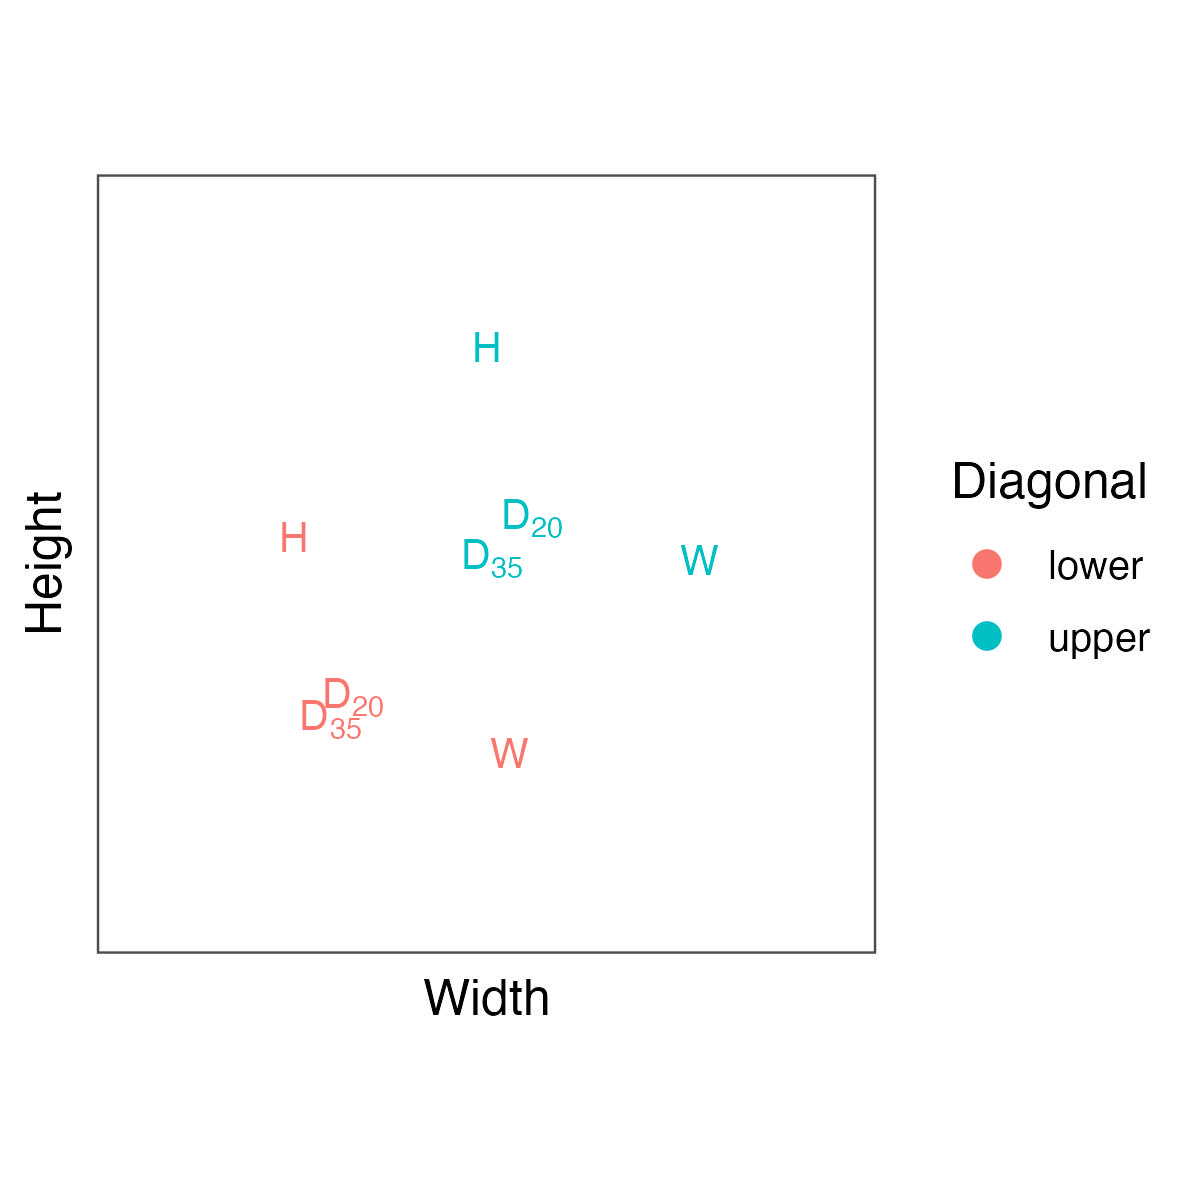
\includegraphics[width=100mm]{figures/comparability_stim.jpg}
   \caption{Graphical depiction of critical stimuli from Experiment 5. The stimuli fall on two diagonals, referred to as upper and lower. The H rectangles are taller than wide, while the W rectangles are wider than tall. The decoy (D) rectangles are equally wide and tall (i.e., squares). The decoy subscripts indicate the $TDD$ $\%$.}
   \label{fig:comparability_stim_plot}
\end{figure}

% On each critical trial, there were three options: an $H$ rectangle, a $W$ rectangle, and a $D$ rectangle. The focal rectangles fell on two diagonals (upper and lower, see above), while the decoy rectangle varied in $TDD$ at $20\%$ and $35\%$. 

The stimuli were arranged in one of four displays: all-aligned, two-aligned, none-aligned, or triangle. See Figure~\ref{fig:comparability_trials} for sample trials. 

In the all-aligned display, all stimuli were arranged in a horizontal array, as in the experiments of \textcite{trueblood2013not} and \textcite{spektorWhenGoodLooks2018b}, Experiment 4.

In the two-aligned display, two options were aligned horizontally in the top-left and top-middle positions, while the third option was placed in the bottom-right position of the screen. This is a crucial condition and an instantiation of the comparability hypothesis, in which the comparison of the two aligned options was far easier than all other pairwise comparisons.

In the none-aligned display, all options are located in different vertical and horizontal positions, such that all comparisons should be more difficult, as determining the relative areas between rectangles is less straightforward.

The triangle display was identical to the triangle display of Experiments 1 and 2, with the exception that on half of all triangle display trials, the triangle was inverted. Note that this condition is distinct from the two aligned condition, as the options were located in distinct vertical and horizontal positions, and it was difficult to determine the relative sizes between rectangles. 
% The triangle display condition was collected for future analyses but is not germane to the current research question, and it will be excluded from critical analyses.

In all displays, the horizontal distances between all options was constant.

In addition to varying diagonal, $TDD$, and display, option order also varied, such that all six orders ($DHW$, $DWH$, $HDW$, $HWD$, $WDH$, and $WHD$) were equally common.

\begin{figure}
   \begin{center}
      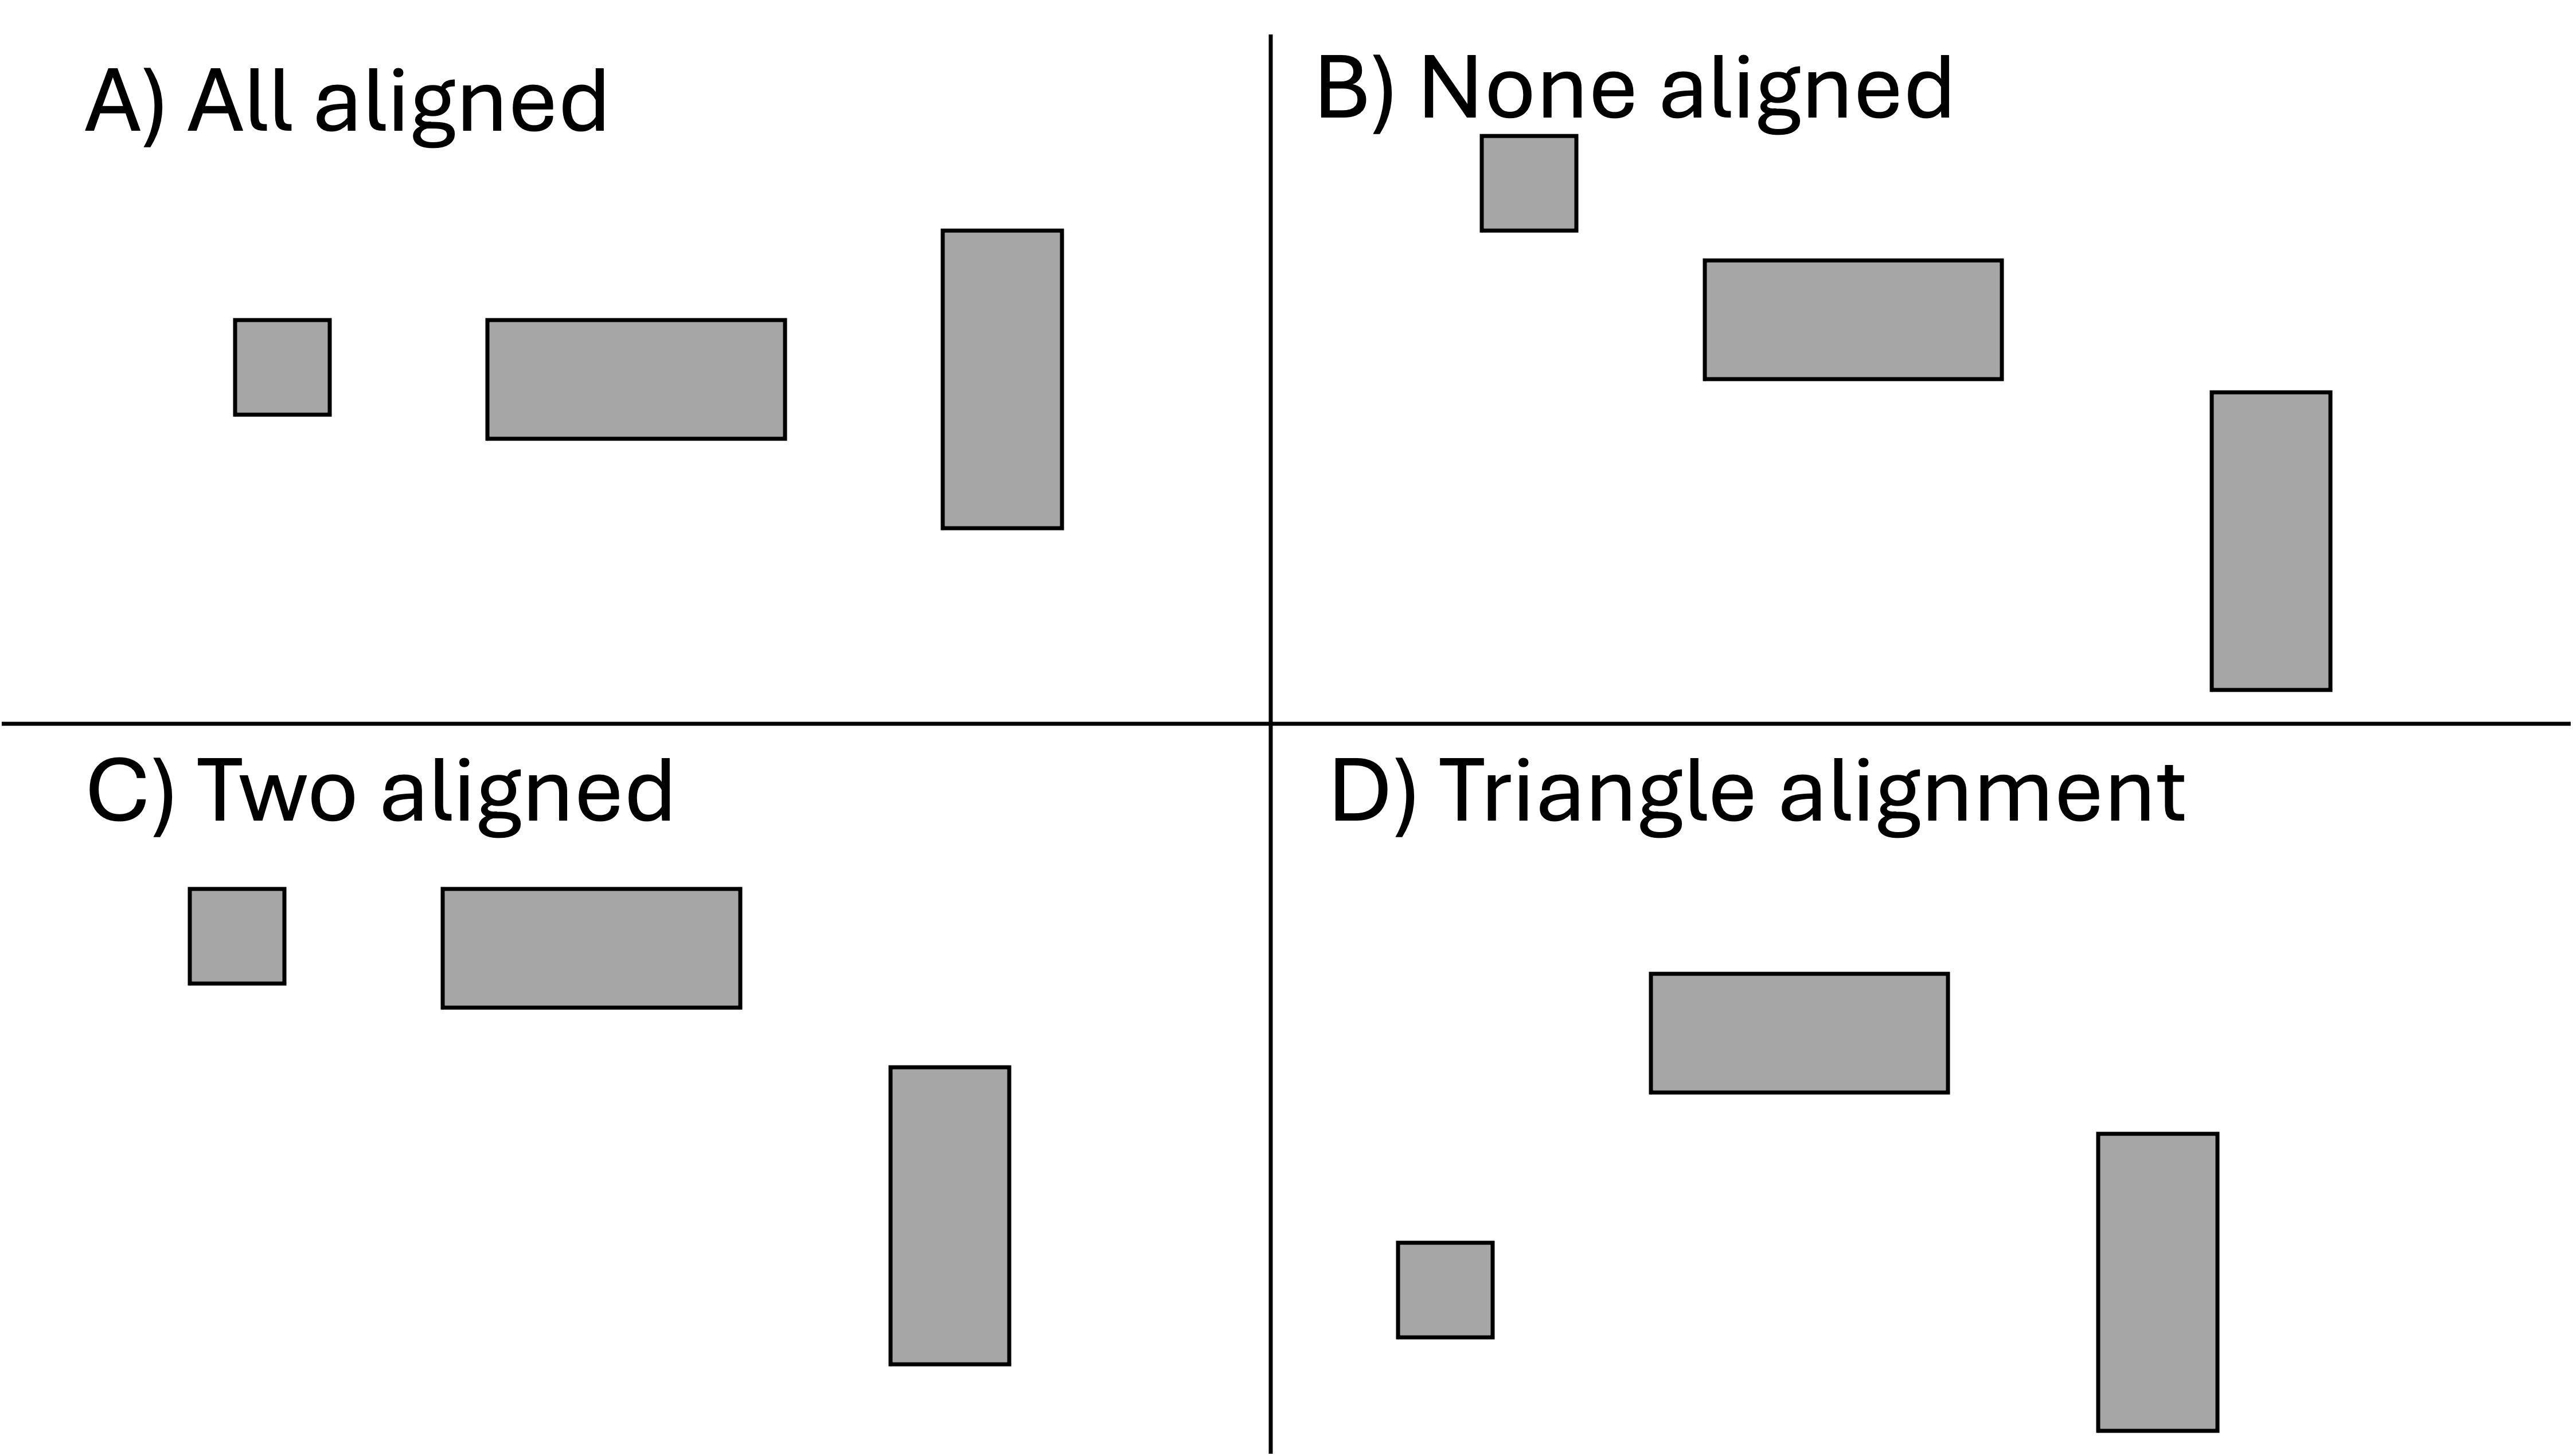
\includegraphics[width=100mm]{figures/comparability_design.jpg}
      \caption{Sample critical trials from Experiment 5. A) all aligned. B) Two aligned. C) None aligned. D) Triangle alignment.}
      \label{fig:comparability_trials}
   \end{center}
\end{figure}

There were other types of stimuli on non-critical trials: filler-random, filler-square, and catch.

On filler-random trials, three options were randomly generated by independently sampling both a height and width from the $U(57,200)px$ distribution. Filler-random trials were included to avoid participants noticing the manipulation on the critical trials and to include enough challenging trials to keep participants engaged in the task.

On filler-square trials, a square was randomly generated by sampling a side length from the $U(57,200)px$ distribution. Then, two non-square rectangles were generated by sampling a height and width from the $U(57,S)px$ distribution, where $S$ is the side length of the square. This procedure ensured that the square was always the largest option on filler-square trials. Filler-square trials were included to ensure that participants did not learn to ignore the squares, as the critical trials rely on participants comparing the squares to the focal options. 

On catch trials, one large option was randomly generated by randomly sampling a stimulus from the upper diagonal (see Figure~\ref{fig:comparability_stim_plot}). Two smaller options were randomly sampled from the lower diagonal. 

\subsubsection{Design}
As discussed above, there were four types of trials: critical trials, filler-square trials, filler-random trials, and catch trials. The study took place in four blocks.

This was a $2$ (diagonal: lower, upper) x $2$ ($TDD$: $20\%$, $35\%$) x $4$ (display: all-aligned, two-aligned, none-aligned, triangle) x $6$ (order: $DHW$, $DWH$, $HDW$, $HWD$, $WDH$, and $WHD$) within-participants study. Each participant completed $4$ trials for all combinations of these factors ($1$ per each of the four blocks), except for the two-aligned trials, for which they completed $8$ trials ($2$ per each of the four blocks). Thus, there were a total of $480$ critical trials ($(2*2*3*6*4)+ (2*2*1*6*8)=480$).

On each of the non-critical trials, stimulus order was randomized. Additionally, one of the four displays (all-aligned, two-aligned, none-aligned, triangle) was selected at random.

There were $40$ filler-random trials per block for each of four blocks, a total of $160$ filler-random trials. There were $40$ filler-square trials per block for each of four blocks, a total of $160$ filler-square trials. There were $10$ catch trials per block for each of four blocks, a total of $40$ catch trials.

There were $840$ total trials in the experiment ($480$ critical $+$ $160$ filler-random $+$ $160$ filler-square $+$ $40$ catch=$840$).

\subsubsection{Procedure}
On each trial, participants saw three rectangles, labeled $1$, $2$, and $3$. Participants were told to select the largest rectangle. They made their choice by pressing the corresponding key on the keyboard. 

The experiment was split into four blocks. There was a 15-second break between blocks.

\subsection{Results}

\subsubsection{Data Processing}
In addition to removing participants who failed to meet the $80\%$ correct criterion for catch trials, $2,319$ trials with RTs $<100ms$ or $>10,000ms$ were removed from all analyses. 

\subsubsection{Catch and Filler Trials}
On average, participants performed well above chance on the catch, filler-random, and filler-square trials, including on all display types. See Figure~\ref{fig:comparability_non_crit_mean_prop_correct} for these data.

\begin{figure}
   \centering
   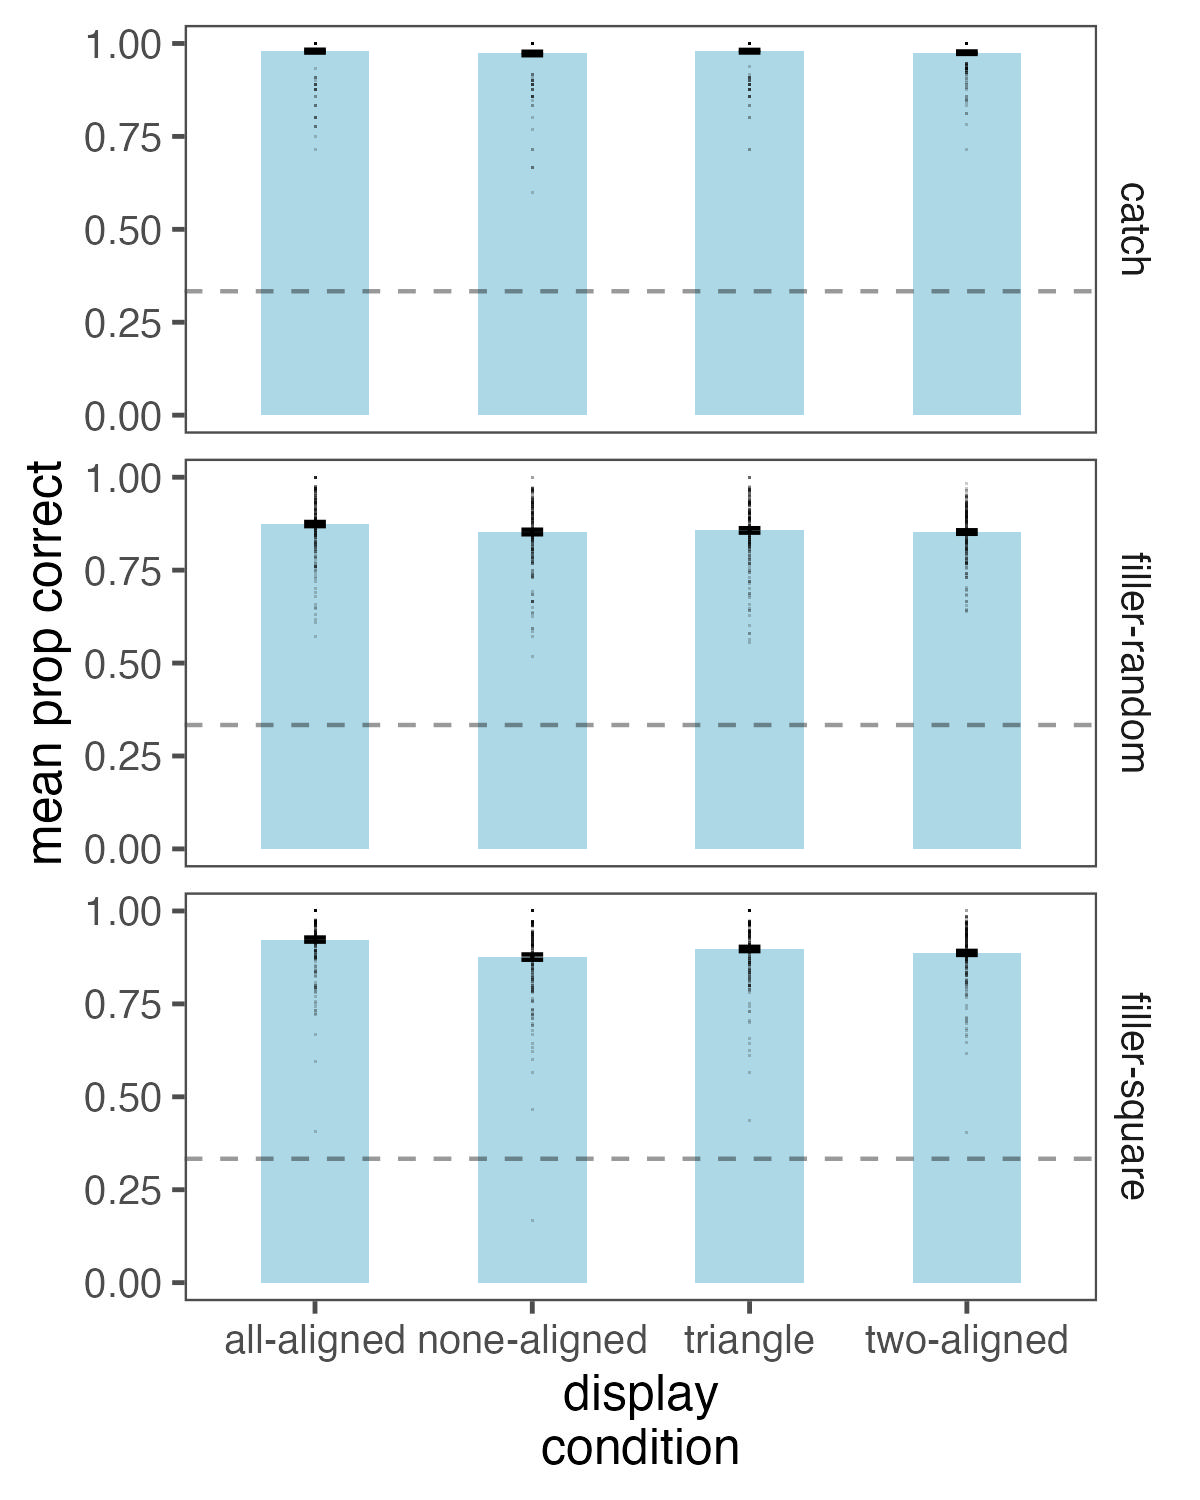
\includegraphics[width=100mm]{figures/non_crit_mean_prop_correct.jpeg}
   \caption{Results from non-critical trials in Experiment 5. Rows show trial types. Bars show mean proportion correct in a given condition, with the error bars showing $\pm1\;\text{SEM}$. Dots show individual participant data. Dashed line is at $1/3$ (chance performance).}
   \label{fig:comparability_non_crit_mean_prop_correct}
\end{figure}

As will be relevant below, participants showed position biases. The order of stimuli on each trial was random, so on average, participants should be equally likely to select the left, middle, rightmost rectangle. However, participants tended to select the middle rectangle the most, followed by the rightmost rectangle, followed by the leftmost rectangle. This bias occurred in each display condition. Mean choice proportions for each position for all non-critical trials (collapsed across trial type) are plotted in Figure~\ref{fig:comparability_pos_bias}.

\begin{figure}
   \centering
   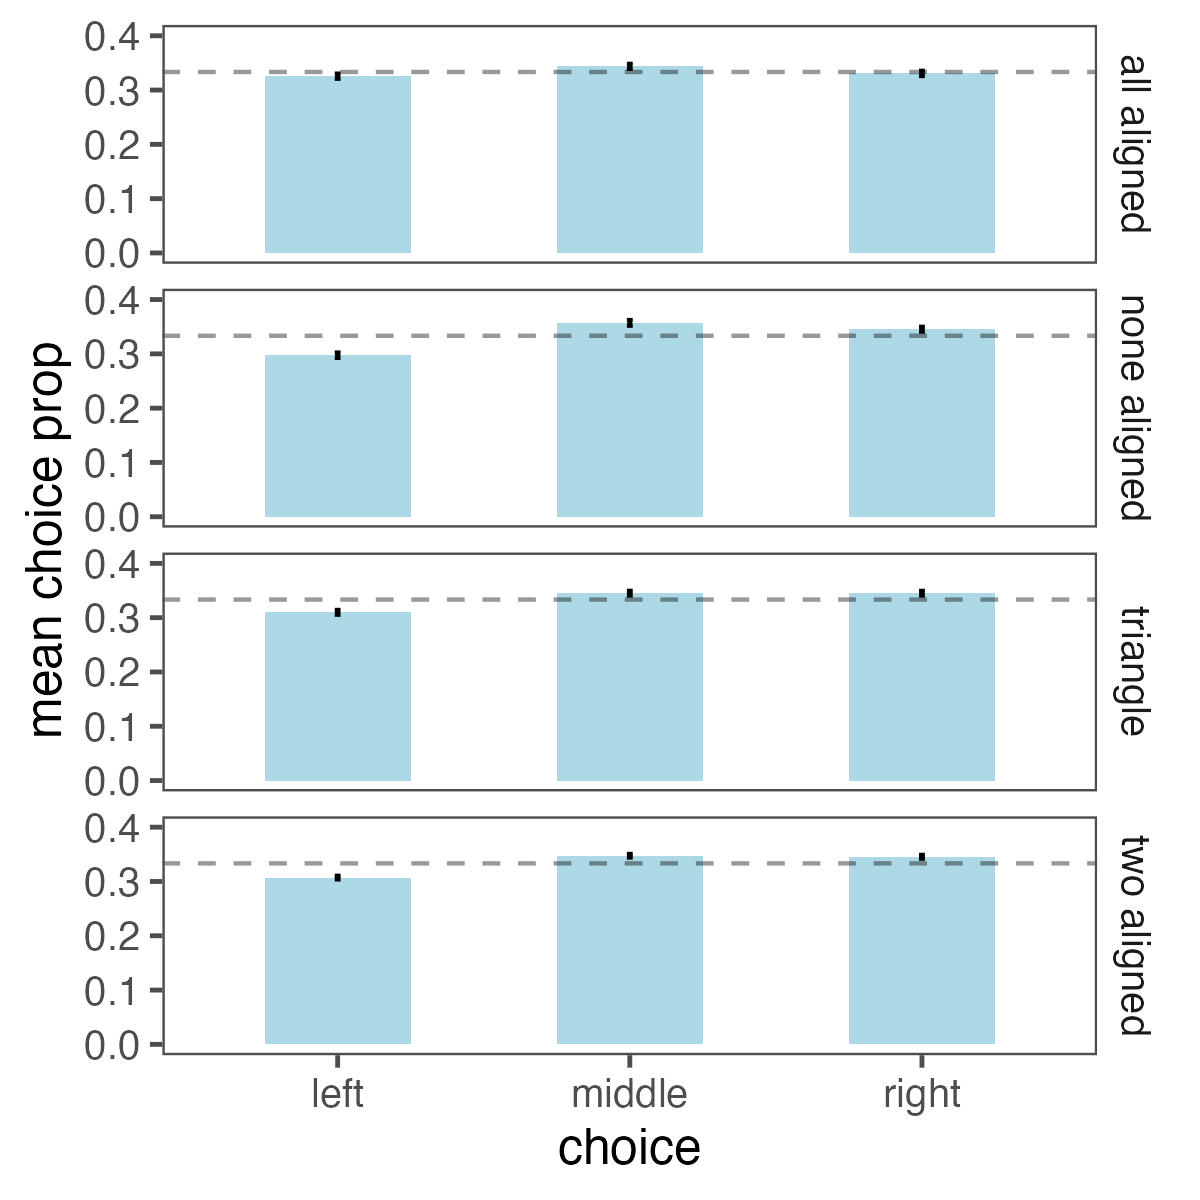
\includegraphics[width=100mm]{figures/comparability_filler_position_bias.jpeg}
   \caption{Position biases from non-critical trials in Experiment 5. Rows show trial types. Bars show mean choice proportions for a given position, with the error bars showing $\pm1\;\text{SEM}$. Dashed line is at chance ($1/3$).}
   \label{fig:comparability_pos_bias}
\end{figure}


\subsubsection{Critical Trials}

The goal of the critical trial analysis was to determine how alignment affected choice for the target option, defined as the rectangle located next to the decoy.

Consider the order of options on screen. There were six possible orderings: $DHW$, $DWH$, $HDW$, $HWD$, $WDH$, and $WHD$. Given that the crucial display is the two-aligned display - where the first two options were aligned vertically while a third option was unaligned both vertically and horizontally - the crucial trials were those trials where the decoy was among the first two options. 

The ordering was re-classified into a variable referred to as alignment. Because the two-aligned condition is the critical one, the alignment variable is labeled based on the order in the two-aligned condition. If the ordering is $DHW$ or $HDW$, the alignment is "$H$ aligned with $D$". If the ordering is $WDH$ or $DWH$, the alignment is "$D$ aligned with $W$". The $WHD$ and $HWD$ trials were removed from further analysis.

The mean choice proportion for the $H$, $W$, and $D$ rectangles based on alignment were computed and are shown in Figure~\ref{fig:comparability_crit_mean_choices}. The data show that, in the two-aligned condition, participants were less likely to choose the $W$ option when it was aligned with $D$ than when $H$ was aligned with $D$. This effect also appears to occur in the none-aligned and all-aligned conditions, which suggests a position bias because choosing $H$ more when $W$ is aligned with $D$ but choosing $W$ more when $H$ is aligned with $D$ amounts to having a bias for the third (rightmost) rectangle.

\begin{figure}
   \centering
   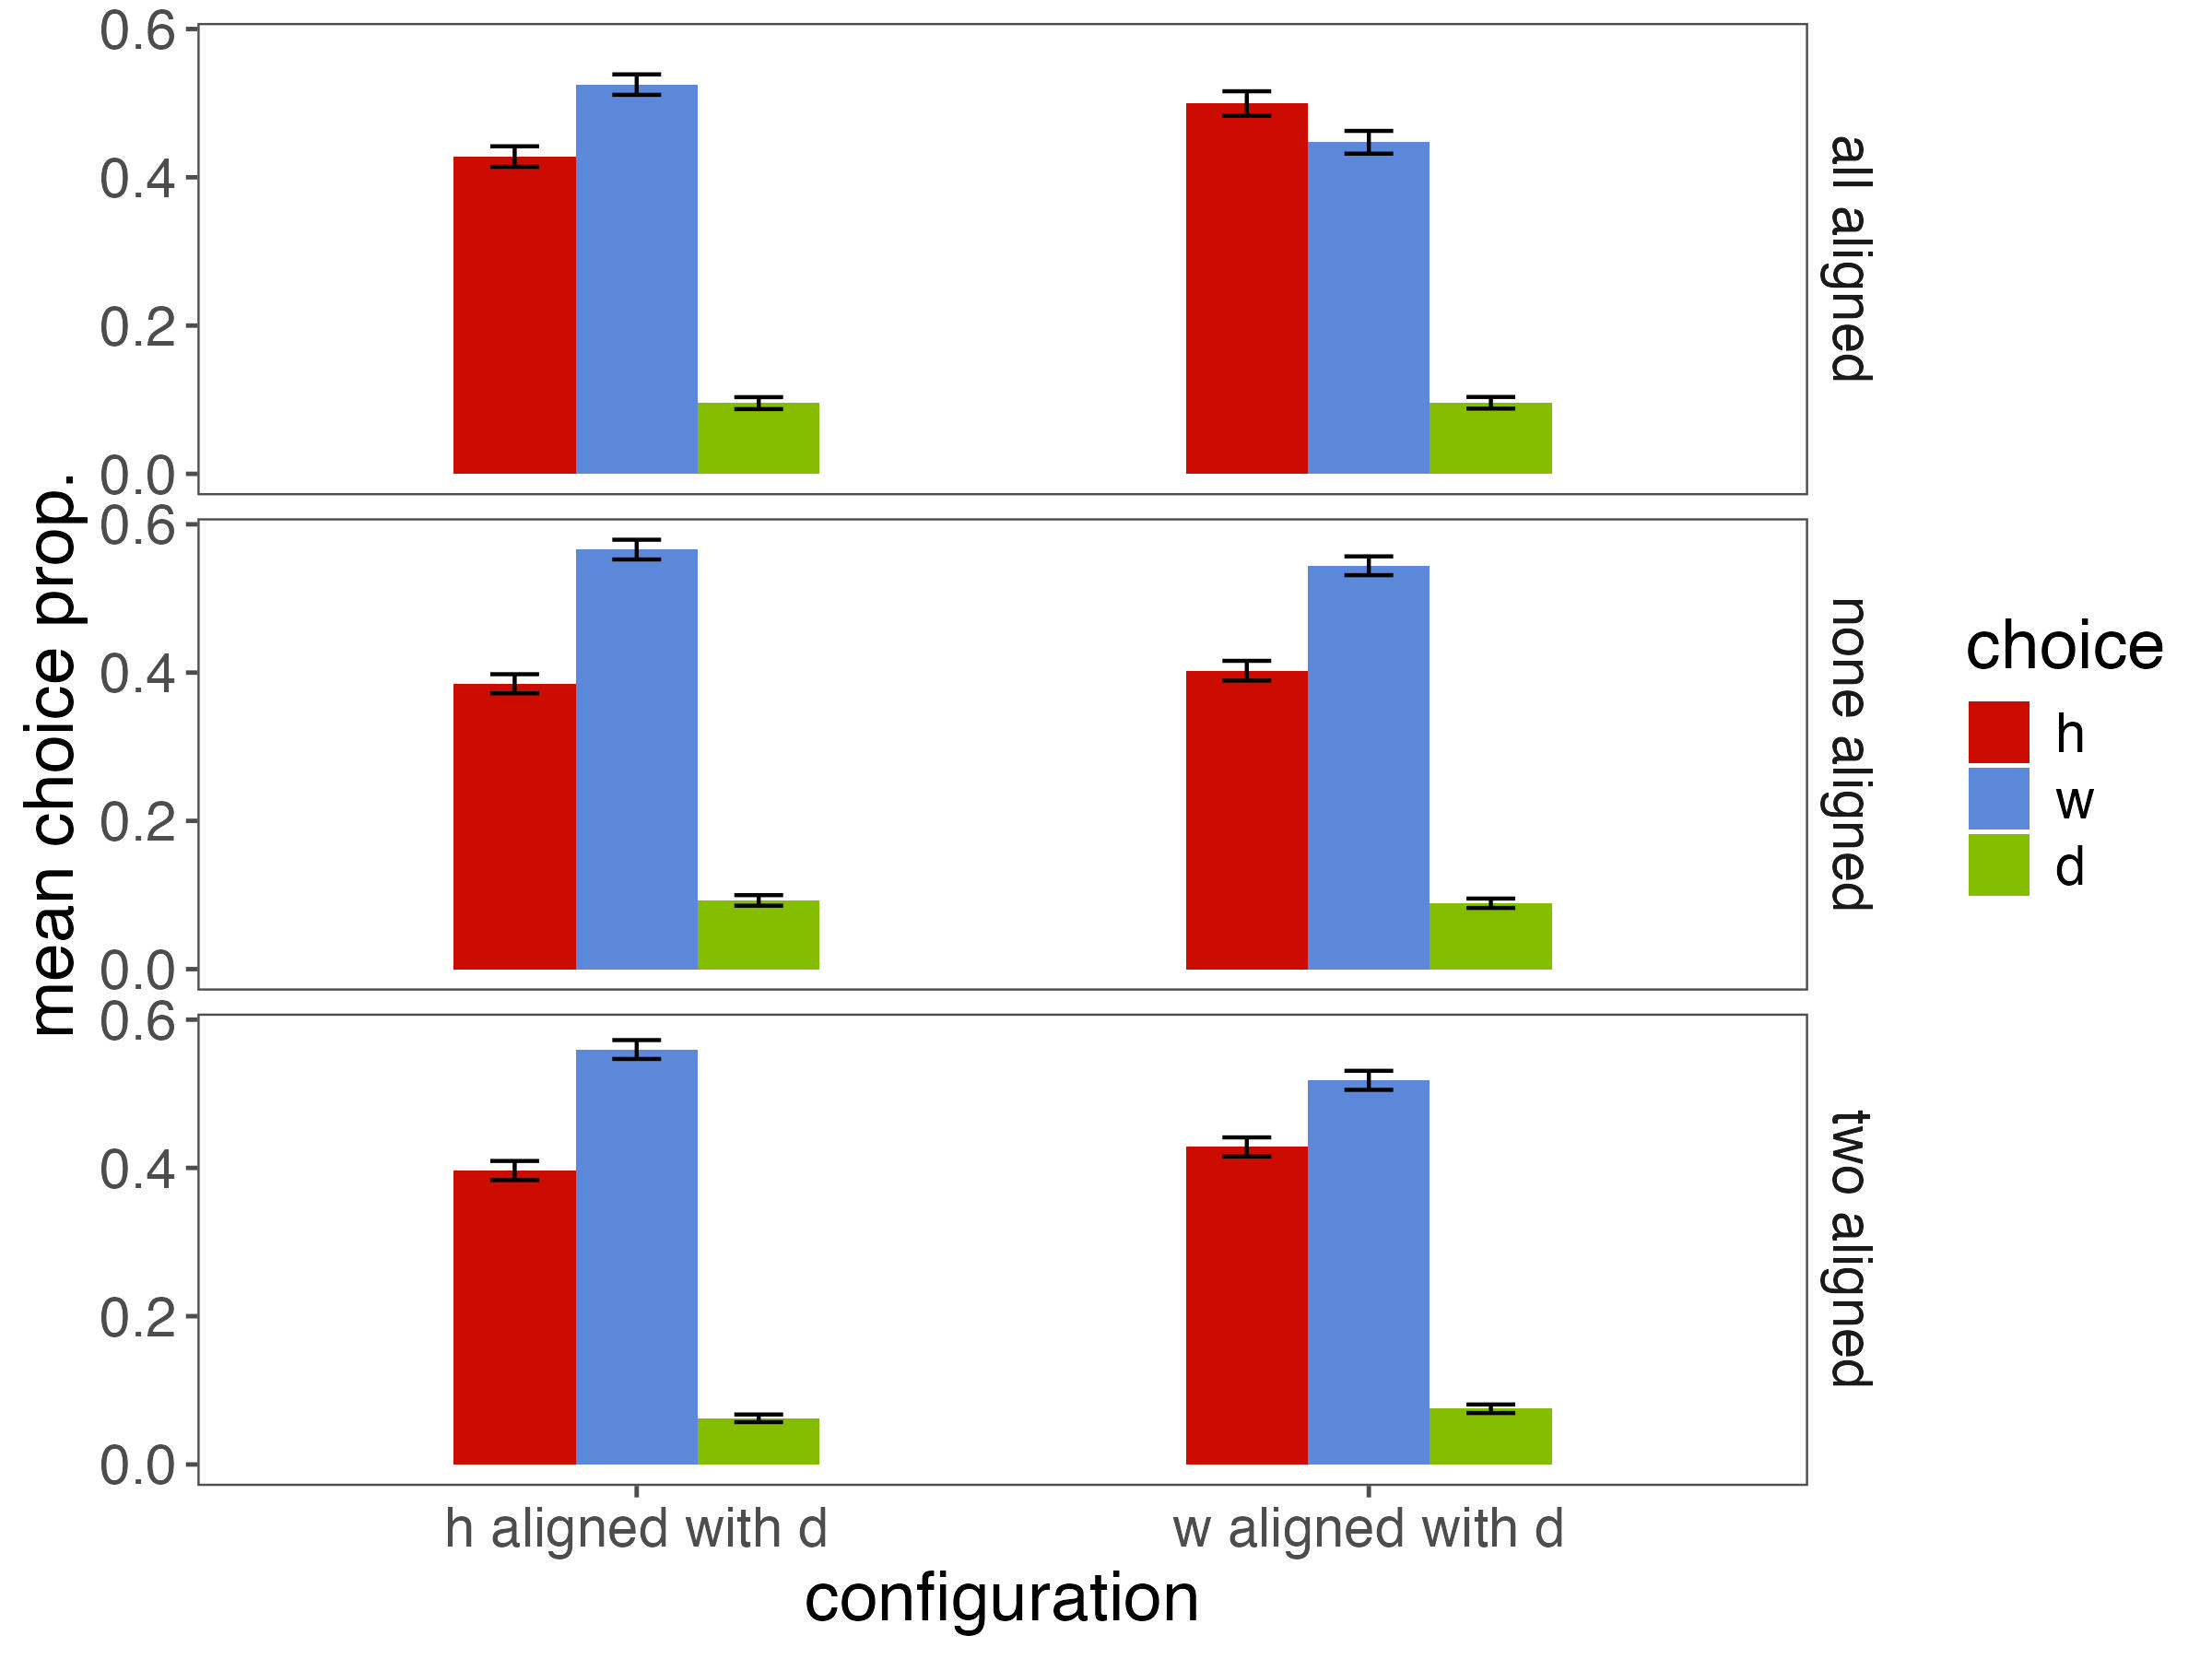
\includegraphics[width=100mm]{figures/comparability_crit_mean_hdw_choice_by_config_align.jpeg}
   \caption{Results from critical trials in Experiment 5. Mean choice proportions for the $H$, $W$, and $D$ rectangles conditioned on alignment and display. Error bars are $\pm1\mathrm{SEM}$.}
   \label{fig:comparability_crit_mean_choices}
\end{figure}

Next, the analyses were collapsed over $H$/$W$ and instead, choices were re-classified into target, competitor, and decoy. The target was the option aligned with the decoy, while the competitor was the option not aligned with the decoy. The decoy label did not change. Mean choice proportions were computed and plotted in Figure~\ref{fig:comparability_crit_mean_tcd_choices}. Note that this classification is most appropriate for the two-aligned condition; the other conditions are included as a point of comparison.

Participants reliably chose the competitor more than the target; however, this effect appears to be stronger in the triangle condition, followed by the all aligned condition, the two aligned condition, and then the none aligned condition. Given that the triangle condition does not readily facilitate comparison between the decoy and the target, choosing the competitor more often in the triangle condition amounts to a bias for the third (rightmost) rectangle. A similar interpretation can be made for the none aligned condition. 

\begin{figure}
   \centering
   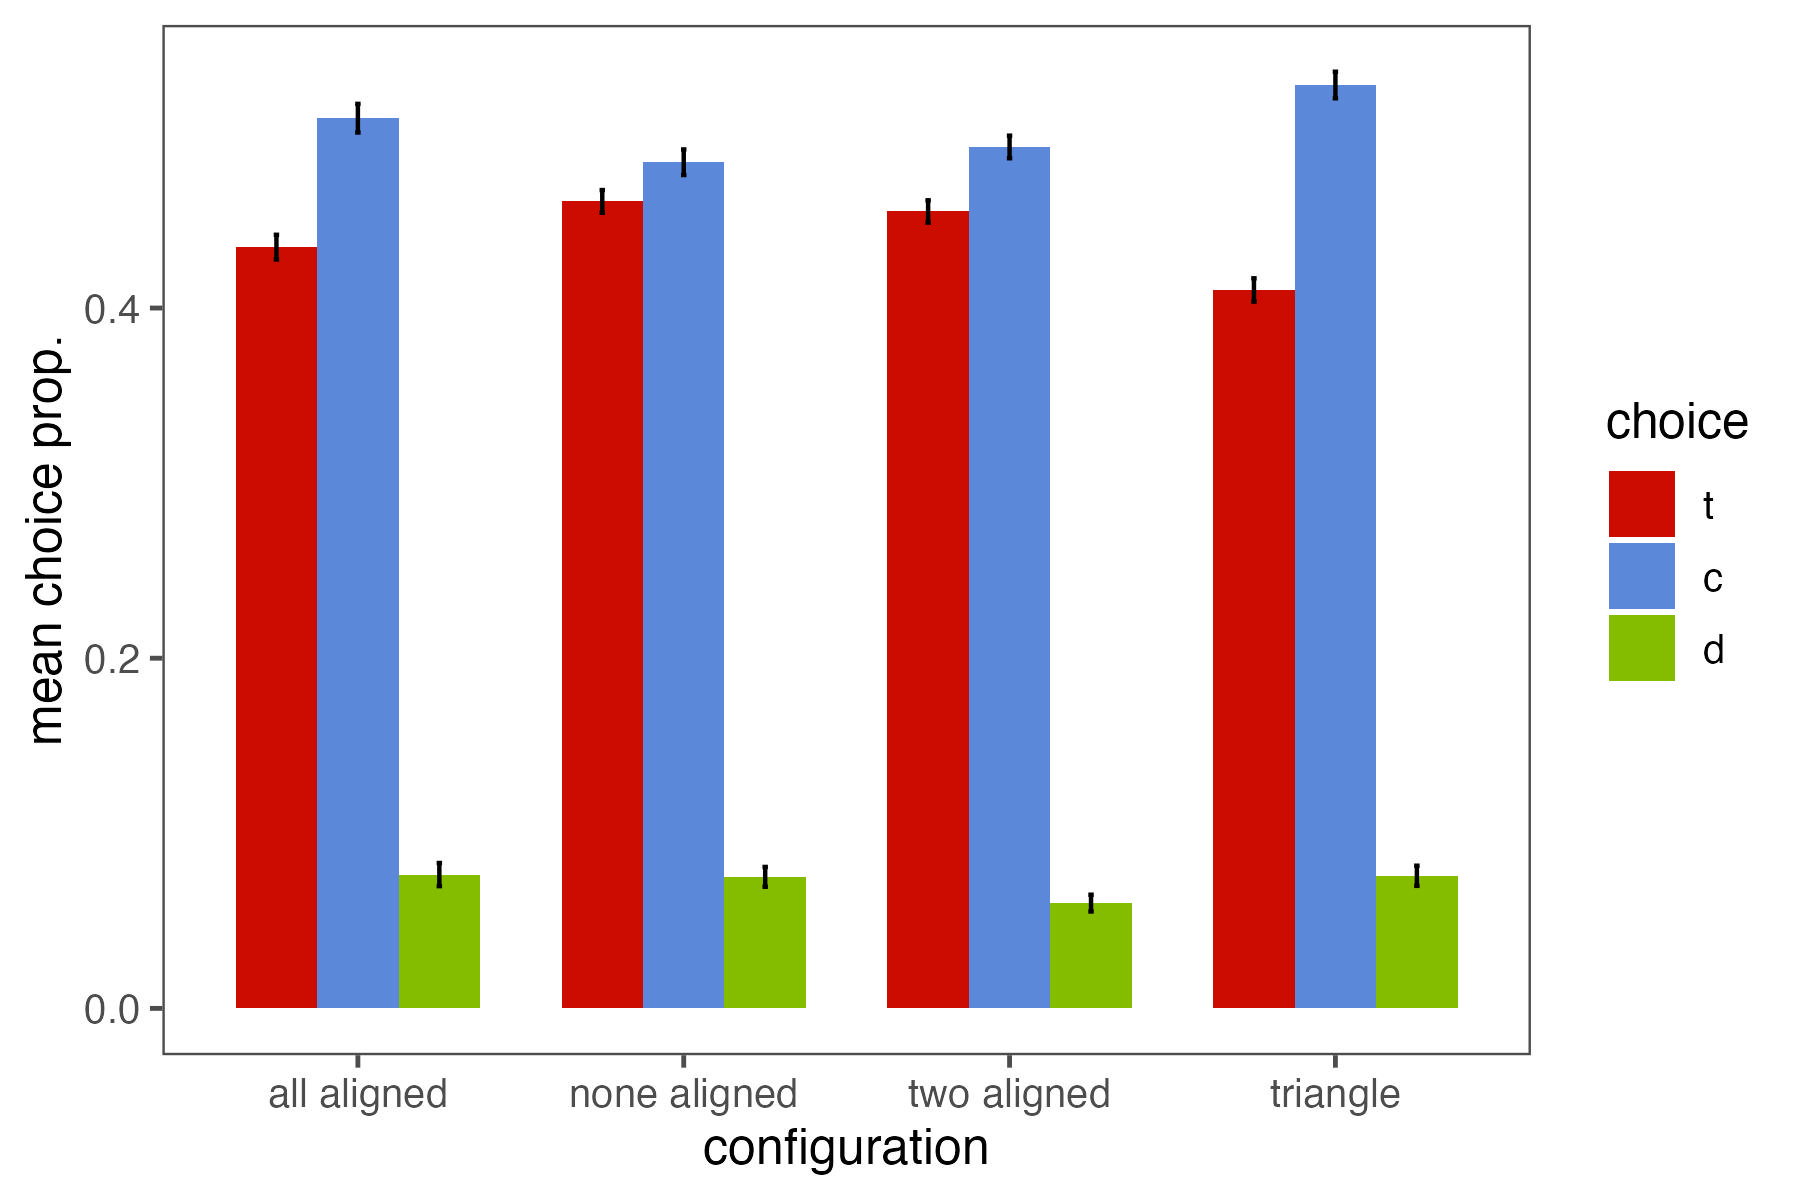
\includegraphics[width=100mm]{figures/comparability_crit_choice_by_config.jpeg}
   \caption{Experiment 5 mean target, competitor, and decoy choice proportions by display. Error bars are $\pm1\mathrm{SEM}$.}
   \label{fig:comparability_crit_mean_tcd_choices}
\end{figure}

Next, all trials in which participants chose the decoy were removed and Relative Share of the Target (RST) was computed. The mean RST is plotted in Figure~\ref{fig:comparability_crit_mean_target_choices}.

\begin{figure}
   \centering
   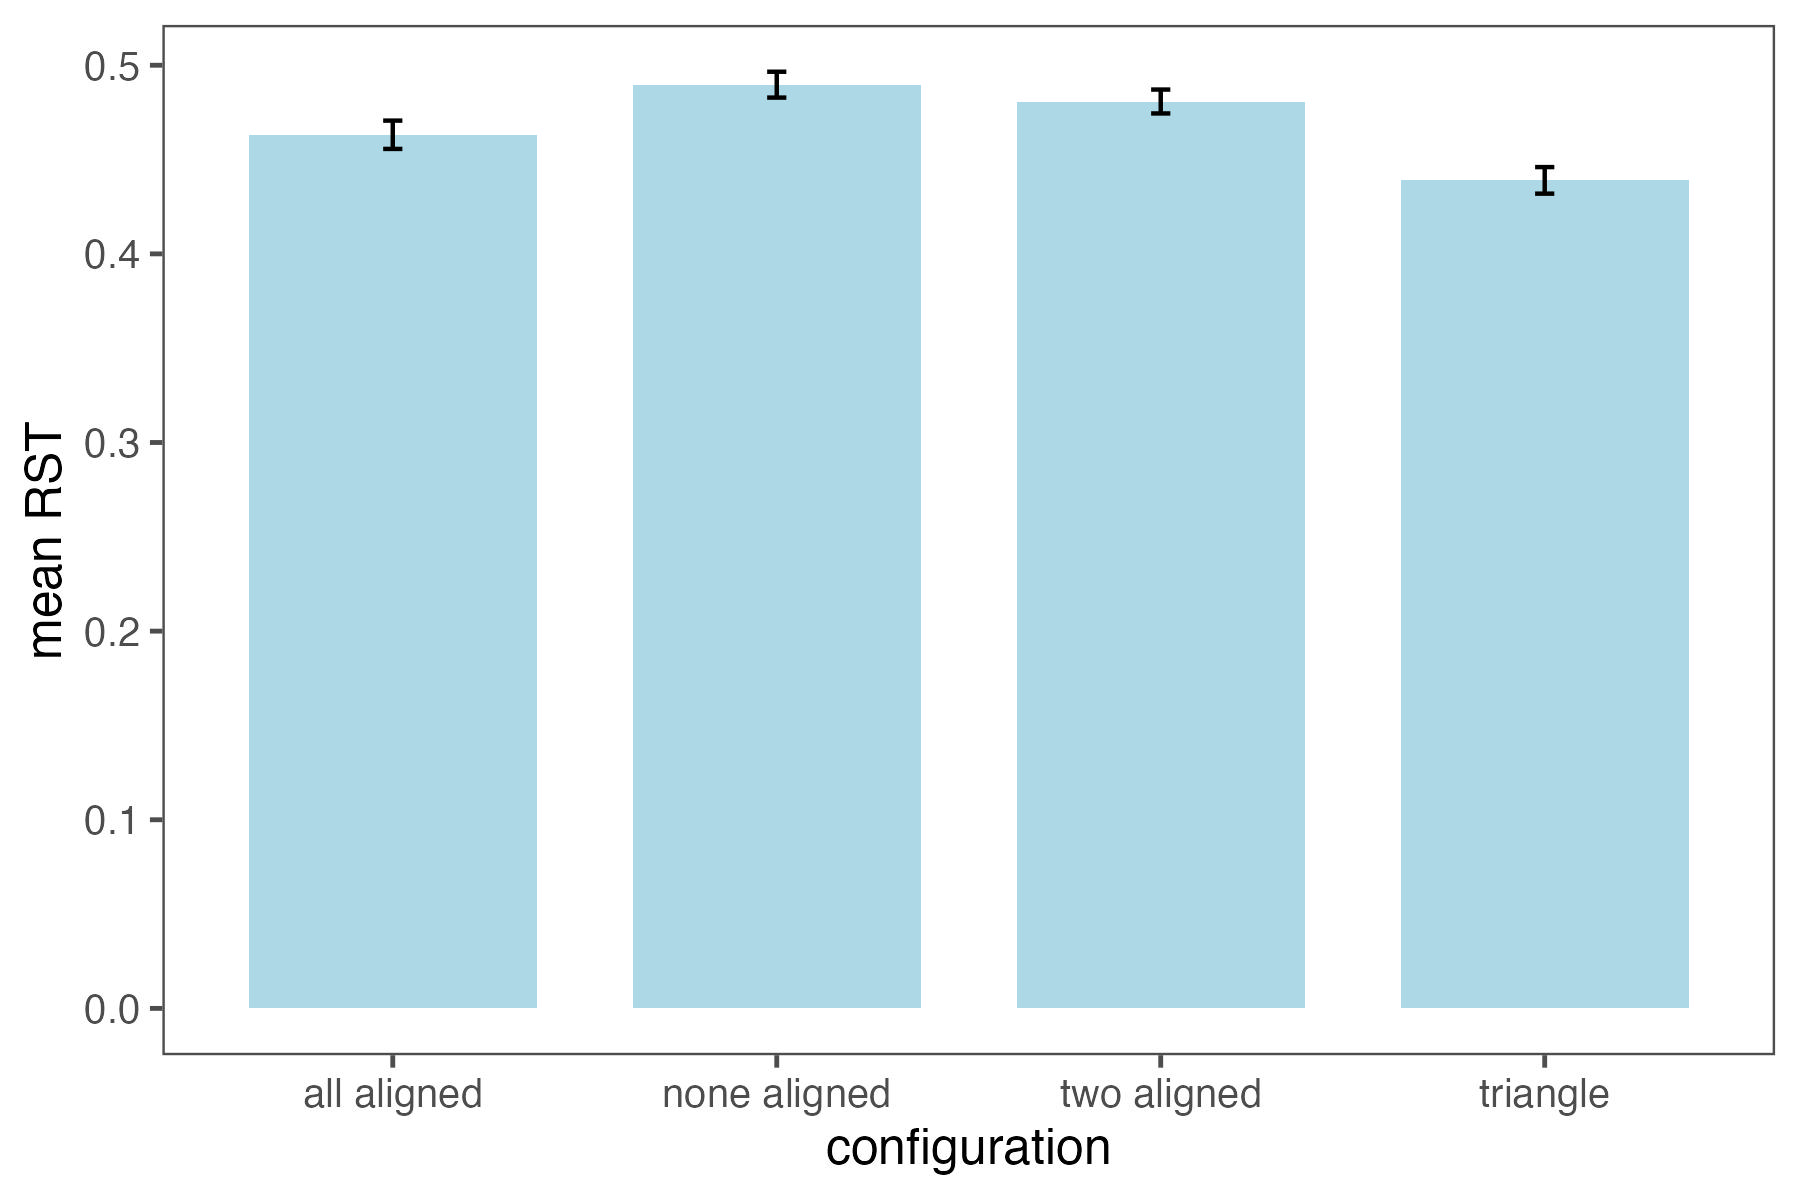
\includegraphics[width=100mm]{figures/comparability_crit_rst_by_config.jpeg}
   \caption{Experiment 5 mean RST by display. Error bars are $\pm1\mathrm{SEM}$.}
   \label{fig:comparability_crit_mean_target_choices}
\end{figure}

On average, participants selected the target option on less than $1/2$ of trials (conditional on not having selected the decoy). This again may suggest a position bias; that is, participants appeared to have a bias for the third (rightmost rectangle) in the choice set. However, crucially, they selected the target less when it is aligned with the decoy in the two-aligned condition than when it is adjacent to the decoy in the none-aligned condition. See the Appendix for inferential statistics which support these conclusions.

\section{Discussion}

Experiment 5 showed that comparability can affect choice. Given two equally viable dissimilar options, when one of these options (i.e., the target) was more easily comparable to a symmetrically dominated decoy option, participants chose the target less than the competitor. This effect is small but nonetheless present.

This result aligns with the predictions from the Thurstonian perceptual choice model from Chapter 2. Increasing the comparability of a focal option and a decoy option increases the perceptual correlations between the two, which in turn decreases the choice share of the comparable \textit{target}, for the benefit of the non-comparable competitor option. This result is also similar to previous results presented by \textcite{trueblood2022attentional} and \textcite{evansImpactPresentationOrder2021}, who also manipulated the arrangement of options on screen in perceptual choice.

These results are, however, somewhat limited by the positioning of the target and decoy options. In the two-aligned condition, the target and decoy were always presented in the first and second position. The statistical model accounted for this through a position bias effect, though a more thorough design would include a variety of presentation formats to more effectively test this effect.

Predictions were made assuming that increasing comparability decreased target choice share through perceptual correlation; however, given that these correlations were not measured directly, this may not be the case. It would be interesting to use the paradigm from Experiment 2 to directly measure the correlations between options when the decoy is symmetrically dominated and the comparability is systematically manipulated.

Future research should generalize this paradigm to high-level preferential choice. For example, given three consumer products, does the comparability of two of them affect the choice for a third option? For example, given three cars available for purchase, two of which are hybrids and the other is a traditional combustion engine vehicle, is the correlation between the hybrids stronger than the hybrid-combustion correlation? This question is left for future research.

When perceptual decisions are difficult, and a decoy option is easily comparable to one of two viable options, this viable option is chosen less than it otherwise would have been chosen. The effect was predicted using the Thurstonian model developed earlier in this dissertation, and the empirical results support it, albeit with limitations.  The empirical results of Experiment 5 demonstrate another form of context dependence, the main focus of this dissertation. Here, the context is not the choice set (which remains constant), but rather the presentation of the options. In this sense, the repulsion effect in this experiment is qualitatively similar to the repulsion effect of \textcite{spektorWhenGoodLooks2018b} and Experiment 2 of this dissertation.
